%%%%%%%%%%%%%%%%%%%%%%%%%%%%%%%%%%%%%%%%%%%%%%%%%%%%%%%%%%%%%%%%%%%%%%%%%%%%%%%%
% Thesis / Project Report
% LaTeX Template
% Version 2.0 (08/04/16)
%
% Author:
% Parth Ganeriwala
% https://github.com/ParthGaneriwala/BITS-Thesis-Template-Latex
%
% This template is heavily based on the work of Siddhant Shrivastava, Darshit Shah, Steven Gunn and Sunil Patel
% Siddhant Shrivastava
% https://github.com/sidcode/bits-pilani-thesis-template-latex
% Darshit Shah
% https://github.com/darnir/BPHC-LaTeX-Report-Class
% Steven Gunn
% http://users.ecs.soton.ac.uk/srg/softwaretools/document/templates/
% and
% Sunil Patel
% http://www.sunilpatel.co.uk/thesis-template/
%
% License:
% CC BY-NC-SA 4.0 (http://creativecommons.org/licenses/by-nc-sa/4.0/)
%
% Note:
% Make sure to edit document variables in the Thesis.cls file
%
%%%%%%%%%%%%%%%%%%%%%%%%%%%%%%%%%%%%%%%%%%%%%%%%%%%%%%%%%%%%%%%%%%%%%%%%%%%%%%%%

%-------------------------------------------------------------------------------
%	PACKAGES AND OTHER DOCUMENT CONFIGURATIONS
%-------------------------------------------------------------------------------

\documentclass[11pt, a4paper, oneside]{Thesis} % Paper size, default font size
                                               % and one-sided paper

\graphicspath{{Pictures/}} % Specifies the directory where pictures are stored

\usepackage[backend=bibtex]{biblatex}
\bibliography{Bibliography.bib}


\title{\ttitle} % Defines the thesis title - don't touch this

\begin{document}

\frontmatter % Use roman numbering style (i, ii...) for the pre-content pages

\setstretch{1.3} % Line spacing of 1.3

% Define page headers using FancyHdr package and set up for one-sided printing
\fancyhead{} % Clears all page headers and footers
\rhead{\thepage} % Sets the right side header to show the page number
\lhead{} % Clears the left side page header

\pagestyle{fancy} % Finally, use the "fancy" page style to implement the
                  %FancyHdr headers

% Input all the variables used in the document. Please fill out the
% variables.tex file with all your details.
%-------------------------------------------------------------------------------
%	DOCUMENT VARIABLES
%
%	Fill in the lines below to set the various variables for the document
%-------------------------------------------------------------------------------

%-------------------------------------------------------------------------------
% Your thesis title - this is used in the title and abstract
% Command: \ttitle
\thesistitle{Enter Your Thesis Title}
%-------------------------------------------------------------------------------
% The document type: Thesis / report, etc.
% Command: \doctype
\documenttype{Undergraduate Thesis}
%-------------------------------------------------------------------------------
% Your supervisor's name - this is used in the title page
% Command: \supname
\supervisor{First Name \textsc{Last Name}}
%-------------------------------------------------------------------------------
% The supervisor's position - Used on Certificate
% Command: \suppos
\supervisorposition{Associate Professor}
%-------------------------------------------------------------------------------
% Supervisor's institute
% Command: \supinst
\supervisorinstitute{BITS Pilani, Dubai Campus}
\supervisorinstitutecountry{United Arab Emirates}
%-------------------------------------------------------------------------------
% Your Co-Supervisor's name
% Command: \cosupname
\cosupervisor{First Name \textsc{Last Name}}
%-------------------------------------------------------------------------------
% Co-Supervisor's Position - Used on Certificate
% Command: \cosuppos
\cosupervisorposition{Associate Professor}
%-------------------------------------------------------------------------------
% Co-Supervisor's Institute
% Command: \cosupinst
\cosupervisorinstitute{}
\cosupervisorinstitutecountry{}
%-------------------------------------------------------------------------------
% Your Examiner's name. Not currently used anywhere.
% Command: \examname
\examiner{}
%-------------------------------------------------------------------------------
% Name of your degree
% Command: \degreename
\degree{Bachelor of Engineering (Hons.)}
%-------------------------------------------------------------------------------
% The BITS Course Code for which this report is written
% COmmand: \ccode
\coursecode{BITS F421T}
%-------------------------------------------------------------------------------
% The name of the Course
% Command: \cname
\coursename{Thesis}
%-------------------------------------------------------------------------------
% Your name. Extend manually in case of multiple authors
% Command: \authornames
\authors{ First Name \textsc{Last Name}}
%-------------------------------------------------------------------------------
% Your ID Number - used on the Title page and abstract
% Command: \idnum
\IDNumber{2018A7TS0XXXU}
%-------------------------------------------------------------------------------
% Your address
% Command: \addressnames
\addresses{}
%-------------------------------------------------------------------------------
% Your subject area
% Command: \subjectname
\subject{}
%-------------------------------------------------------------------------------
% Keywords for this report.
% Command: \keywordnames
\keywords{}
%-------------------------------------------------------------------------------
% University details
% Command: \univname
\university{\texorpdfstring{\href{https://www.bits-pilani.ac.in/Dubai/index.aspx} % URL
                {Birla Institute of Technology and Science Pilani, Dubai Campus}} % University name
                {Birla Institute of Technology and Science Pilani, Dubai Campus}}
%-------------------------------------------------------------------------------
% University details, in Capitals
% Command: \UNIVNAME
\UNIVERSITY{\texorpdfstring{\href{https://www.bits-pilani.ac.in/Dubai/index.aspx} % URL
                {Birla Institute Of Technology And Science Pilani, Dubai Campus}} % name in capitals
                {Birla Institute Of Technology And Science Pilani, Dubai Campus}}
                
\UNIVERSITYCOUNTRY{\texorpdfstring{Dubai, U.A.E}}
%-------------------------------------------------------------------------------
% Department Details
% Command: \deptname
\department{\texorpdfstring{\href{https://www.bits-pilani.ac.in/dubai/computerscience/DetofComputerScience} % Your department's URL
                {Computer Science}} % Your department's name
                {Computer Science}}
%-------------------------------------------------------------------------------
% Department details, in Capitals
% Command: \DEPTNAME
\DEPARTMENT{\texorpdfstring{\href{https://www.bits-pilani.ac.in/dubai/computerscience/DetofComputerScience} % Your department's URL
                {Computer Science}} % Your department's name in capitals
                {Computer Science}}
%-------------------------------------------------------------------------------
% Research Group Details
% Command: \groupname
\group{\texorpdfstring{\href{Research Group Web Site URL Here (include http://)}
                {Research Group Name}} % Your research group's name
                {Research Group Name}}
%-------------------------------------------------------------------------------
% Research Group Details, in Capitals
% Command: \GROUPNAME
\GROUP{\texorpdfstring{\href{Research Group Web Site URL Here (include http://)}
                {RESEARCH GROUP NAME (IN BLOCK CAPITALS)}}
                {RESEARCH GROUP NAME (IN BLOCK CAPITALS)}}
%-------------------------------------------------------------------------------
% Faculty details
% Command: \facname
\faculty{\texorpdfstring{\href{Faculty Web Site URL Here (include http://)}
                {Faculty Name}}
                {Faculty Name}}
%-------------------------------------------------------------------------------
% Faculty details, in Capitals
% Command: \FACNAME
\FACULTY{\texorpdfstring{\href{Faculty Web Site URL Here (include http://)}
                {FACULTY NAME (IN BLOCK CAPITALS)}}
                {FACULTY NAME (IN BLOCK CAPITALS)}}
%-------------------------------------------------------------------------------


%-------------------------------------------------------------------------------
%   NON-CONTENT PAGES
%-------------------------------------------------------------------------------
\maketitle
\Declaration
\Certificate
% \Quotation{Insert Random Quote here. Publish like a boss.}{Your Name}

\begin{abstract}
The Thesis Abstract is written here (and usually kept to just this page).
The page is kept centered vertically so it can expand into the blank space above
the title too\ldots

\end{abstract}

\begin{acknowledgements}

The acknowledgements and the people to thank go here, don't forget to include your project advisor and friends\ldots

\vspace{2cm}
Signed:\\
\rule[1em]{25em}{0.5pt} % This prints a line for the signature

\authornames\\
ID No. \idnum\\
\end{acknowledgements}

%-------------------------------------------------------------------------------
%	LIST OF CONTENTS/FIGURES/TABLES PAGES
%-------------------------------------------------------------------------------

% The page style headers have been "empty" all this time, now use the "fancy"
% headers as defined before to bring them back
\pagestyle{fancy}

\lhead{\emph{Contents}} % Set the left side page header to "Contents"
\tableofcontents % Write out the Table of Contents

% Set the left side page header to "List of Figures"
\lhead{\emph{List of Figures}}
\listoffigures % Write out the List of Figures

 % Set the left side page header to "List of Tables"
\lhead{\emph{List of Tables}}
\listoftables % Write out the List of Tables

%-------------------------------------------------------------------------------
%	ABBREVIATIONS
%-------------------------------------------------------------------------------

\clearpage % Start a new page

 % Set the line spacing to 1.5, this makes the following tables easier to read
\setstretch{1.5}

\lhead{\emph{Abbreviations}} % Set the left side page header to "Abbreviations"
\listofsymbols{ll} % Include a list of Abbreviations (a table of two columns)
{
\textbf{LAH} & \textbf{L}ist \textbf{A}bbreviations \textbf{H}ere \\
%\textbf{Acronym} & \textbf{W}hat (it) \textbf{S}tands \textbf{F}or \\
}

%-------------------------------------------------------------------------------
%	PHYSICAL CONSTANTS/OTHER DEFINITIONS
%-------------------------------------------------------------------------------

% \clearpage % Start a new page

% % Set the left side page header to "Physical Constants"
% \lhead{\emph{Physical Constants}}

%  % Include a list of Physical Constants (a four column table)
% \listofconstants{lrcl}
% {
% Speed of Light & $c$ & $=$ & $2.997\ 924\ 58\times10^{8}\ \mbox{ms}^{-\mbox{s}}$ (exact)\\
% % Constant Name & Symbol & = & Constant Value (with units) \\
% }

%-------------------------------------------------------------------------------
%	SYMBOLS
%-------------------------------------------------------------------------------

% \clearpage % Start a new page

% \lhead{\emph{Glossary}} % Set the left side page header to "Symbols"

% \listofnomenclature % List the nomenclature. (We use the glossaries package)

%-------------------------------------------------------------------------------
%	DEDICATION
%-------------------------------------------------------------------------------

\setstretch{1.3} % Return the line spacing back to 1.3

\pagestyle{empty} % Page style needs to be empty for this page

% Dedication text
\Dedicatory{Dedicate this to someone, anyone.}

\addtocontents{toc}{\vspace{2em}} % Add a gap in the Contents, for aesthetics

%-------------------------------------------------------------------------------
%	THESIS CONTENT - CHAPTERS
%-------------------------------------------------------------------------------

\mainmatter % Begin numeric (1,2,3...) page numbering

\pagestyle{fancy} % Return the page headers back to the "fancy" style

% Include the chapters of the thesis as separate files from the Chapters folder
% Uncomment the lines as you write the chapters

% Chapter 1

\chapter{Chapter Title Here} % Main chapter title

\label{Chapter1} % For referencing the chapter elsewhere, use \ref{Chapter1} 

\lhead{Chapter 1. \emph{Chapter Title Here}} % This is for the header on each page - perhaps a shortened title

%----------------------------------------------------------------------------------------

\section{Welcome and Thank You}
Welcome to this \LaTeX{} Thesis Template, a beautiful and easy to use template for writing a thesis using the \LaTeX{} typesetting system.

If you are writing a thesis (or will be in the future) and its subject is technical or mathematical (though it doesn't have to be), then creating it in \LaTeX{} is highly recommended as a way to make sure you can just get down to the essential writing without having to worry over formatting or wasting time arguing with your word processor.

\LaTeX{} is easily able to professionally typeset documents that run to hundreds or thousands of pages long. With simple mark-up commands, it automatically sets out the table of contents, margins, page headers and footers and keeps the formatting consistent and beautiful. One of its main strengths is the way it can easily typeset mathematics, even \emph{heavy} mathematics. Even if those equations are the most horribly twisted and most difficult mathematical problems that can only be solved on a super-computer, you can at least count on \LaTeX{} to make them look stunning.

%----------------------------------------------------------------------------------------

\section{Learning \LaTeX{}}

\LaTeX{} is not a WYSIWYG (What You See is What You Get) program, unlike word processors such as Microsoft Word or Apple's Pages. Instead, a document written for \LaTeX{} is actually a simple, plain text file that contains \emph{no formatting}. You tell \LaTeX{} how you want the formatting in the finished document by writing in simple commands amongst the text, for example, if I want to use \textit{italic text for emphasis}, I write the `$\backslash$\texttt{textit}\{\}' command and put the text I want in italics in between the curly braces. This means that \LaTeX{} is a ``mark-up'' language, very much like HTML.

\subsection{A (not so short) Introduction to \LaTeX{}}

If you are new to \LaTeX{}, there is a very good eBook -- freely available online as a PDF file -- called, ``The Not So Short Introduction to \LaTeX{}''. The book's title is typically shortened to just ``lshort''. You can download the latest version (as it is occasionally updated) from here:\\
\href{http://www.ctan.org/tex-archive/info/lshort/english/lshort.pdf}{\texttt{http://www.ctan.org/tex-archive/info/lshort/english/lshort.pdf}}

It is also available in several other languages. Find yours from the list on this page:\\
\href{http://www.ctan.org/tex-archive/info/lshort/}{\texttt{http://www.ctan.org/tex-archive/info/lshort/}}

It is recommended to take a little time out to learn how to use \LaTeX{} by creating several, small `test' documents. Making the effort now means you're not stuck learning the system when what you \emph{really} need to be doing is writing your thesis.

\subsection{A Short Math Guide for \LaTeX{}}

If you are writing a technical or mathematical thesis, then you may want to read the document by the AMS (American Mathematical Society) called, ``A Short Math Guide for \LaTeX{}''. It can be found online here:\\
\href{http://www.ams.org/tex/amslatex.html}{\texttt{http://www.ams.org/tex/amslatex.html}}\\
under the ``Additional Documentation'' section towards the bottom of the page.

\subsection{Common \LaTeX{} Math Symbols}
There are a multitude of mathematical symbols available for \LaTeX{} and it would take a great effort to learn the commands for them all. The most common ones you are likely to use are shown on this page:\\
\href{http://www.sunilpatel.co.uk/latexsymbols.html}{\texttt{http://www.sunilpatel.co.uk/latexsymbols.html}}

You can use this page as a reference or crib sheet, the symbols are rendered as large, high quality images so you can quickly find the \LaTeX{} command for the symbol you need.

\subsection{\LaTeX{} on a Mac}
 
The \LaTeX{} package is available for many systems including Windows, Linux and Mac OS X. The package for OS X is called MacTeX and it contains all the applications you need -- bundled together and pre-customised -- for a fully working \LaTeX{} environment and workflow.
 
MacTeX includes a dedicated \LaTeX{} IDE (Integrated Development Environment) called ``TeXShop'' for writing your `\texttt{.tex}' files and ``BibDesk'': a program to manage your references and create your bibliography section just as easily as managing songs and creating playlists in iTunes.

%----------------------------------------------------------------------------------------

\section{Getting Started with this Template}

If you are familiar with \LaTeX{}, then you can familiarise yourself with the contents of the Zip file and the directory structure and then place your own information into the `\texttt{Thesis.cls}' file. Section \ref{FillingFile} on page \pageref{FillingFile} tells you how to do this. Make sure you read section \ref{ThesisConventions} about thesis conventions to get the most out of this template and then get started with the `\texttt{Thesis.tex}' file straightaway.

If you are new to \LaTeX{} it is recommended that you carry on reading through the rest of the information in this document.

\subsection{About this Template}

This \LaTeX{} Thesis Template is originally based and created around a \LaTeX{} style file created by Steve R.\ Gunn from the University of Southampton (UK), department of Electronics and Computer Science. You can find his original thesis style file at his site, here:\\
\href{http://www.ecs.soton.ac.uk/~srg/softwaretools/document/templates/}{\texttt{http://www.ecs.soton.ac.uk/$\sim$srg/softwaretools/document/templates/}}

My thesis originally used the `\texttt{ecsthesis.cls}' from his list of styles. However, I knew \LaTeX{} could still format better. To get the look I wanted, I modified his style and also created a skeleton framework and folder structure to place the thesis files in.

This Thesis Template consists of that modified style, the framework and the folder structure. All the work that has gone into the preparation and groundwork means that all you have to bother about is the writing.

Before you begin using this template you should ensure that its style complies with the thesis style guidelines imposed by your institution. In most cases this template style and layout will be suitable. If it is not, it may only require a small change to bring the template in line with your institution's recommendations.

%----------------------------------------------------------------------------------------

\section{What this Template Includes}

\subsection{Folders}

This template comes as a single Zip file that expands out to many files and folders. The folder names are mostly self-explanatory:

\textbf{Appendices} -- this is the folder where you put the appendices. Each appendix should go into its own separate `\texttt{.tex}' file. A template is included in the directory.

\textbf{Chapters} -- this is the folder where you put the thesis chapters. A thesis usually has about seven chapters, though there is no hard rule on this. Each chapter should go in its own separate `\texttt{.tex}' file and they usually are split as:
\begin{itemize}
\item Chapter 1: Introduction to the thesis topic
\item Chapter 2: Background information and theory
\item Chapter 3: (Laboratory) experimental setup
\item Chapter 4: Details of experiment 1
\item Chapter 5: Details of experiment 2
\item Chapter 6: Discussion of the experimental results
\item Chapter 7: Conclusion and future directions
\end{itemize}
This chapter layout is specialised for the experimental sciences.

\textbf{Figures} -- this folder contains all figures for the thesis. These are the final images that will go into the thesis document.

\textbf{Primitives} -- this is the folder that contains scraps, particularly because one final image in the `Figures' folder may be made from many separate images and photos, these source images go here. This keeps the intermediate files separate from the final thesis figures.

\subsection{Files}

Included are also several files, most of them are plain text and you can see their contents in a text editor. Luckily, many of them are auxiliary files created by \LaTeX{} or BibTeX and which you don't need to bother about:

\textbf{Bibliography.bib} -- this is an important file that contains all the bibliographic information and references that you will be citing in the thesis for use with BibTeX. You can write it manually, but there are reference manager programs available that will create and manage it for you. Bibliographies in \LaTeX{} are a large subject and you may need to read about BibTeX before starting with this.

\textbf{Thesis.cls} -- this is an important file. It is the style file that tells \LaTeX{} how to format the thesis. You will also need to open this file in a text editor and fill in your own information (such as name, department, institution). Luckily, this is not too difficult and is explained in section \ref{FillingFile} on page \pageref{FillingFile}.

\textbf{Thesis.pdf} -- this is your beautifully typeset thesis (in the PDF file format) created by \LaTeX{}.

\textbf{Thesis.tex} -- this is an important file. This is the file that you tell \LaTeX{} to compile to produce your thesis as a PDF file. It contains the framework and constructs that tell \LaTeX{} how to layout the thesis. It is heavily commented so you can read exactly what each line of code does and why it is there. After you put your own information into the `\texttt{Thesis.cls}' file, go to this file and begin filling it in -- you have now started your thesis!

\textbf{vector.sty} -- this is a \LaTeX{} package, it tells \LaTeX{} how to typeset mathematical vectors. Using this package is very easy and you can read the documentation on the site (you just need to look at the `\texttt{vector.pdf}' file):\\
\href{http://www.ctan.org/tex-archive/macros/latex/contrib/vector/}{\texttt{http://www.ctan.org/tex-archive/macros/latex/contrib/vector/}}

\textbf{lstpatch.sty} -- this is a \LaTeX{} package required by this LaTeX template and is included as not all \TeX{} distributions have it installed by default. You do not need to modify this file.

Files that are \emph{not} included, but are created by \LaTeX{} as auxiliary files include:

\textbf{Thesis.aux} -- this is an auxiliary file generated by \LaTeX{}, if it is deleted \LaTeX{} simply regenerates it when you run the main `\texttt{.tex}' file.

\textbf{Thesis.bbl} -- this is an auxiliary file generated by BibTeX, if it is deleted, BibTeX simply regenerates it when you run the main tex file. Whereas the `\texttt{.bib}' file contains all the references you have, this `\texttt{.bbl}' file contains the references you have actually cited in the thesis and is used to build the bibliography section of the thesis.

\textbf{Thesis.blg} -- this is an auxiliary file generated by BibTeX, if it is deleted BibTeX simply regenerates it when you run the main `\texttt{.tex}' file.

\textbf{Thesis.lof} -- this is an auxiliary file generated by \LaTeX{}, if it is deleted \LaTeX{} simply regenerates it when you run the main `\texttt{.tex}' file. It tells \LaTeX{} how to build the `List of Figures' section.

\textbf{Thesis.log} -- this is an auxiliary file generated by \LaTeX{}, if it is deleted \LaTeX{} simply regenerates it when you run the main `\texttt{.tex}' file. It contains messages from \LaTeX{}, if you receive errors and warnings from \LaTeX{}, they will be in this `\texttt{.log}' file.

\textbf{Thesis.lot} -- this is an auxiliary file generated by \LaTeX{}, if it is deleted \LaTeX{} simply regenerates it when you run the main `\texttt{.tex}' file. It tells \LaTeX{} how to build the `List of Tables' section.

\textbf{Thesis.out} -- this is an auxiliary file generated by \LaTeX{}, if it is deleted \LaTeX{} simply regenerates it when you run the main `\texttt{.tex}' file.


So from this long list, only the files with the `\texttt{.sty}', `\texttt{.bib}', `\texttt{.cls}' and `\texttt{.tex}' extensions are the most important ones. The other auxiliary files can be ignored or deleted as \LaTeX{} and BibTeX will regenerate them.

%----------------------------------------------------------------------------------------

\section{Filling in the `\texttt{Thesis.cls}' File}\label{FillingFile}

You will need to personalise the thesis template and make it your own by filling in your own information. This is done by editing the `\texttt{Thesis.cls}' file in a text editor.

Open the file and scroll down, past all the `$\backslash$\texttt{newcommand}\ldots' items until you see the entries for `\texttt{University Name}', `\texttt{Department Name}', etc\ldots.

Fill out the information about your group and institution and ensure you keep to block capitals where it asks you to. You can also insert web links, if you do, make sure you use the full URL, including the `\texttt{http://}' for this.

The last item you should need to fill in is the Faculty Name (in block capitals). When you have done this, save the file and recompile `\texttt{Thesis.tex}'. All the information you filled in should now be in the PDF, complete with web links. You can now begin your thesis proper!

%----------------------------------------------------------------------------------------

\section{The `\texttt{Thesis.tex}' File Explained}

The \texttt{Thesis.tex} file contains the structure of the thesis. There are plenty of written comments that explain what pages, sections and formatting the \LaTeX{} code is creating. Initially there seems to be a lot of \LaTeX{} code, but this is all formatting, and it has all been taken care of so you don't have to do it.

Begin by checking that your information on the title page is correct. For the thesis declaration, your institution may insist on something different than the text given. If this is the case, just replace what you see with what is required.

Then comes a page which contains a funny quote. You can put your own, or quote your favourite scientist, author, person, etc\ldots Make sure to put the name of the person who you took the quote from.

Next comes the acknowledgements. On this page, write about all the people who you wish to thank (not forgetting parents, partners and your advisor/supervisor).

The contents pages, list of figures and tables are all taken care of for you and do not need to be manually created or edited. The next set of pages are optional and can be deleted since they are for a more technical thesis: insert a list of abbreviations you have used in the thesis, then a list of the physical constants and numbers you refer to and finally, a list of mathematical symbols used in any formulae. Making the effort to fill these tables means the reader has a one-stop place to refer to instead of searching the internet and references to try and find out what you meant by certain abbreviations or symbols.

The list of symbols is split into the Roman and Greek alphabets. Whereas the abbreviations and symbols ought to be listed in alphabetical order (and this is \emph{not} done automatically for you) the list of physical constants should be grouped into similar themes.

The next page contains a one line dedication. Who will you dedicate your thesis to?

Finally, there is the section where the chapters are included. Uncomment the lines (delete the `\texttt{\%}' character) as you write the chapters. Each chapter should be written in its own file and put into the `Chapters' folder and named `\texttt{Chapter1}', `\texttt{Chapter2}, etc\ldots Similarly for the appendices, uncomment the lines as you need them. Each appendix should go into its own file and placed in the `Appendices' folder.

After the preamble, chapters and appendices finally comes the bibliography. The bibliography style (called `\texttt{unsrtnat}') is used for the bibliography and is a fully featured style that will even include links to where the referenced paper can be found online. Do not under estimate how grateful you reader will be to find that a reference to a paper is just a click away. Of course, this relies on you putting the URL information into the BibTeX file in the first place.

%----------------------------------------------------------------------------------------

\section{Thesis Features and Conventions}\label{ThesisConventions}

To get the best out of this template, there are a few conventions that you may want to follow.

One of the most important (and most difficult) things to keep track of in such a long document as a thesis is consistency. Using certain conventions and ways of doing things (such as using a Todo list) makes the job easier. Of course, all of these are optional and you can adopt your own method.

\subsection{Printing Format}

This thesis template is designed for single sided printing as most theses are printed and bound this way. This means that the left margin is always wider than the right (for binding). Four out of five people will now judge the margins by eye and think, ``I never 
noticed that before.''.

The headers for the pages contain the page number on the right side (so it is easy to flick through to the page you want) and the chapter name on the left side.

The text is set to 11 point and a line spacing of 1.3. Generally, it is much more readable to have a smaller text size and wider gap between the lines than it is to have a larger text size and smaller gap. Again, you can tune the text size and spacing should you want or need to. The text size can be set in the options for the `$\backslash$\texttt{documentclass}' command at the top of the `\texttt{Thesis.tex}' file and the spacing can be changed by setting a different value in the `$\backslash$\texttt{setstretch}' commands (scattered throughout the `\texttt{Thesis.tex}' file).

\subsection{Using US Letter Paper}

The paper size used in the template is A4, which is a common -- if not standard -- size in Europe. If you are using this thesis template elsewhere and particularly in the United States, then you may have to change the A4 paper size to the US Letter size. Unfortunately, this is not as simple as replacing instances of `\texttt{a4paper}' with `\texttt{letterpaper}'.

This is because the final PDF file is created directly from the \LaTeX{} source using a program called `\texttt{pdfTeX}' and in certain conditions, paper size commands are ignored and all documents are created with the paper size set to the size stated in the configuration file for pdfTeX (called `\texttt{pdftex.cfg}').

What needs to be done is to change the paper size in the configuration file for \texttt{pdfTeX} to reflect the letter size. There is an excellent tutorial on how to do this here: \\
\href{http://www.physics.wm.edu/~norman/latexhints/pdf_papersize.html}{\texttt{http://www.physics.wm.edu/$\sim$norman/latexhints/pdf\_papersize.html}}

It may be sufficient just to replace the dimensions of the A4 paper size with the US Letter size in the \texttt{pdftex.cfg} file. Due to the differences in the paper size, the resulting margins may be different to what you like or require (as it is common for Institutions to dictate certain margin sizes). If this is the case, then the margin sizes can be tweaked by opening up the \texttt{Thesis.cls} file and searching for the line beginning with, `$\backslash$\texttt{setmarginsrb}' (not very far down from the top), there you will see the margins specified. Simply change those values to what you need (or what looks good) and save. Now your document should be set up for US Letter paper size with suitable margins.

\subsection{References}

The `\texttt{natbib}' package is used to format the bibliography and inserts references such as this one \cite{cmu-malware}. The options used in the `\texttt{Thesis.tex}' file mean that the references are listed in numerical order as they appear in the text. Multiple references are rearranged in numerical order (e.g. \cite{kendall2007practical}). This is done automatically for you. To see how you use references, have a look at the `\texttt{Chapter1.tex}' source file. Many reference managers allow you to simply drag the reference into the document as you type.

Scientific references should come \emph{before} the punctuation mark if there is one (such as a comma or period). The same goes for footnotes\footnote{Such as this footnote, here down at the bottom of the page.}. You can change this but the most important thing is to keep the convention consistent throughout the thesis. Footnotes themselves should be full, descriptive sentences (beginning with a capital letter and ending with a full stop).

To see how \LaTeX{} typesets the bibliography, have a look at the very end of this document (or just click on the reference number links).

\subsection{Figures}

There will hopefully be many figures in your thesis (that should be placed in the `Figures' folder). The way to insert figures into your thesis is to use a code template like this:
\begin{verbatim}
\begin{figure}[htbp]
  \centering
    
\includegraphics{Figures/Electron.pdf}
    \rule{35em}{0.5pt}
  \caption[An Electron]{An electron (artist's impression).}
  \label{fig:Electron}
\end{figure}
\end{verbatim}
Also look in the source file. Putting this code into the source file produces the picture of the electron that you can see in the figure below.

\begin{figure}[htbp]
	\centering
		
\includegraphics{Figures/Electron.pdf}
		\rule{35em}{0.5pt}
	\caption[An Electron]{An electron (artist's impression).}
	\label{fig:Electron}
\end{figure}

Sometimes figures don't always appear where you write them in the source. The placement depends on how much space there is on the page for the figure. Sometimes there is not enough room to fit a figure directly where it should go (in relation to the text) and so \LaTeX{} puts it at the top of the next page. Positioning figures is the job of \LaTeX{} and so you should only worry about making them look good!

Figures usually should have labels just in case you need to refer to them (such as in Figure \ref{fig:Electron}). The `$\backslash$\texttt{caption}' command contains two parts, the first part, inside the square brackets is the title that will appear in the `List of Figures', and so should be short. The second part in the curly brackets should contain the longer and more descriptive caption text.

The `$\backslash$\texttt{rule}' command is optional and simply puts an aesthetic horizontal line below the image. If you do this for one image, do it for all of them.

The \LaTeX{} Thesis Template is able to use figures that are either in the PDF or JPEG file format.

\subsection{Typesetting mathematics}

If your thesis is going to contain heavy mathematical content, be sure that \LaTeX{} will make it look beautiful, even though it won't be able to solve the equations for you.

The ``Not So Short Introduction to \LaTeX{}'' (available \href{http://www.ctan.org/tex-archive/info/lshort/english/lshort.pdf}{here}) should tell you everything you need to know for most cases of typesetting mathematics. If you need more information, a much more thorough mathematical guide is available from the AMS called, ``A Short Math Guide to \LaTeX{}'' and can be downloaded from:\\
\href{ftp://ftp.ams.org/pub/tex/doc/amsmath/short-math-guide.pdf}{\texttt{ftp://ftp.ams.org/pub/tex/doc/amsmath/short-math-guide.pdf}}

There are many different \LaTeX{} symbols to remember, luckily you can find the most common symbols \href{http://www.sunilpatel.co.uk/latexsymbols.html}{here}. You can use the web page as a quick reference or crib sheet and because the symbols are grouped and rendered as high quality images (each with a downloadable PDF), finding the symbol you need is quick and easy.

You can write an equation, which is automatically given an equation number by \LaTeX{} like this:
\begin{verbatim}
\begin{equation}
E = mc^{2}
  \label{eqn:Einstein}
\end{equation}
\end{verbatim}

This will produce Einstein's famous energy-matter equivalence equation:
\begin{equation}
E = mc^{2}
\label{eqn:Einstein}
\end{equation}

All equations you write (which are not in the middle of paragraph text) are automatically given equation numbers by \LaTeX{}. If you don't want a particular equation numbered, just put the command, `$\backslash$\texttt{nonumber}' immediately after the equation.

%----------------------------------------------------------------------------------------

\section{Sectioning and Subsectioning}

You should break your thesis up into nice, bite-sized sections and subsections. \LaTeX{} automatically builds a table of Contents by looking at all the `$\backslash$\texttt{chapter}$\{\}$', `$\backslash$\texttt{section}$\{\}$' and `$\backslash$\texttt{subsection}$\{\}$' commands you write in the source.

The table of Contents should only list the sections to three (3) levels. A `$\backslash$\texttt{chapter}$\{\}$' is level one (1). A `$\backslash$\texttt{section}$\{\}$' is level two (2) and so a `$\backslash$\texttt{subsection}$\{\}$' is level three (3). In your thesis it is likely that you will even use a `$\backslash$\texttt{subsubsection}$\{\}$', which is level four (4). Adding all these will create an unnecessarily cluttered table of Contents and so you should use the `$\backslash$\texttt{subsubsection$^{*}\{\}$}' command instead (note the asterisk). The asterisk ($^{*}$) tells \LaTeX{} to omit listing the subsubsection in the Contents, keeping it clean and tidy.

%----------------------------------------------------------------------------------------

\section{In Closing}

You have reached the end of this mini-guide. You can now rename or overwrite this pdf file and begin writing your own `\texttt{Chapter1.tex}' and the rest of your thesis. The easy work of setting up the structure and framework has been taken care of for you. It's now your job to fill it out!
Good luck and have lots of fun!


% % Chapter 2

\chapter{Background Theory} % Main chapter title

\label{Chapter2} % For referencing the chapter elsewhere, use \ref{Chapter1} 

\lhead{Chapter 2. \emph{Background Theory}} % This is for the header on each page - perhaps a shortened title

%------------------------

--------------------------------------------------------------------------

Autonomous vehicular systems are adopting lane detection as a part of their driving assistance systems. Lane detection is to detect lanes on the road and provide the accurate location and shape of each lane. It serves as one of the key techniques to enable modern assisted and autonomous driving systems. One of the principal approaches to lane detection is the accurate detection of road boundaries and lanes using a vision system however it is a difficult problem due to varying road conditions. To train the vision systems for different sets of vehicular systems (aircrafts, motor cycles, cars), huge amounts of dataset are required for the individual systems. We propose a unified machine learning model enhanced by transfer learning which would assist artificial intelligent systems in autonomous driving systems.


\section{Artificial Intelligence}


Artificial intelligence (AI) refers to machines' creative ability to assess data and make intelligent decisions, implying that they can make decisions and perform tasks based on data in the same way that humans do. The world is changing at a rapid pace, with Artificial Intelligence at the forefront of transforming the environment and how we live. AI and self-driving cars are becoming more common in our daily lives and primary industries. It is an area of computer science concerned with intelligent machine behavior and a machine's cleverly simulated ability to mimic human actions and reaction patterns. Artificial intelligence is being more widely used in the field of driving, which is beneficial to driverless vehicles and the Advanced Driver Assistance System (ADAS). For instance, ADAS have been categorized into different levels based on the amount of automation, and the scale provided by The Society of Automotive Engineers (SAE).\cite{8633345} There are five distinguished levels of ADAS. At Level 0, ADAS cannot control the vehicle and can only supply information for the driver to understand on their own. The various examples of Level 0 can be given as parking sensors, surround-view, traffic sign recognition, lane departure warning, night vision, blind spot information system, rear-cross traffic alert, and forward-collision warning. The following Level 1 and 2 are very identical to each other where the driver has the control to make majority of the decision. The only The distinction between the two levels is that Level 1 can manage one capability while Level 2 can control numerous to assist the driver.\cite{8633345}. Some examples of Level 1 ADAS include adaptive cruise control, emergency brake aid, automated emergency brake help, lane maintaining, and lane centering where as Level 2 ADAS include highway aid, autonomous obstacle avoidance, and automated parking. Level 3 to 5 ascends with the increased control of the degree of supervision in accordance to the vehicle with Level 5 being entirely autonomous. Lane detection, as a fundamental challenge in autonomous driving, is crucial in applications including vehicle real-time positioning, driving route planning, lane keeping aid, and adaptive cruise control. 

In terms of both the diversity of potential applications and the levels of interest among conventional actors in the automotive, truck, public transportation, industrial, and military communities, the field of intelligent vehicles is quickly expanding around the world. Intelligent vehicle (IV) solutions have the potential to improve safety and operating efficiency significantly. As a component of intelligent transportation systems (ITS), IV systems use a distinct sensor in conjunction with an intelligent algorithm to analyze the surrounding environment in order to either aid the driver in vehicle operations (driver assistance) or totally operate the vehicle.\cite{1364006}

Modern automobiles include an increasing variety of driver assistance capabilities, like automatic lane maintaining. The latter enables the vehicle to correctly position itself within the road lanes, which is also critical for any later lane departure or trajectory planning choice in fully autonomous vehicles. Traditional lane detection systems rely on a combination of highly specialized, hand-crafted features and heuristics, which are frequently followed by post-processing procedures that are computationally expensive and susceptible to scalability due to road scene fluctuations. Fully autonomous vehicles are currently the primary focus of computer vision and robotics research, both at the academic and industrial levels. The goal in each scenario is to gain a complete understanding of the world around the car by utilizing numerous sensors and control modules. Camera-based lane recognition is a crucial step toward such environmental perception since it allows the car to place itself correctly inside the road lanes. It's also important for each subsequent lane departure or trajectory planning decision. As a result, reliable camera-based lane recognition in real-time is a critical enabler of fully autonomous driving.\cite{neven_towards_2018}

AI is an important factor in this entire equation as it is the decision maker which has been trained based on various selected machine learning algorithms and this process has been enhanced with transfer learning to bring in higher efficiency and precision. 
%----------------------------------------------------------------------------------------

\section{Machine Learning}


Machine learning is a branch of artificial intelligence and computer science that focuses on using data and algorithms to replicate how humans learn, gradually improving its accuracy. Artificial intelligence systems are used to solve complex problems in a way that is similar to how humans solve problems. If an agent improves its decision making with each iteration by retaining information or making observations in the current environment, it is said to be learning. It is the process through which an agent adapts to new situations, discovers, and extrapolates patterns in the given universe. 


The swift and steady development and adoption of high-precision optic and electronic sensors has called for high-efficiency and high-effective computer vision and machine learning algorithms which provide real-time driving scene analysis. Current research has been based on developing advanced algorithms for driving scene interpretation, with the goal of developing either an autonomous car or an advanced driver aid system (ADAS). Prior to the development of self-driving cars, automobiles had Active Lane Tracking Assistance. Because of the scarcity of self-driving cars, several well-known automobile manufacturers adopt this method. This system may be used in a variety of ways. These are just sound and vibration warnings, steering interventions in place of the driver, and so on. This technology aids in keeping the car in its lane. As a result, the significance of lane tracking system is realized.\cite{kamci_lane_2019} Lane detection is one of the most fundamental study areas which has been focused on as part of the autonomous driving aided systems. To develop an artificial intelligent interface, we need machine learning to make it accurate with the highest efficiency and precision. \cite{zou_robust_2020} 




\section{Transfer Learning}

Transfer learning is a useful approach in machine learning for dealing with the fundamental problem of  insufficient training data. It attempts to transfer knowledge from the source domain to the target domain by reducing the requirement that the training and test data be i.i.d. This will have a significant beneficial impact on many areas that are difficult to develop due to a lack of training data. Figure 1 depicts the transfer learning learning process. Some of the terms used in this survey should be defined.


\begin{figure}[htbp]
	\centering
		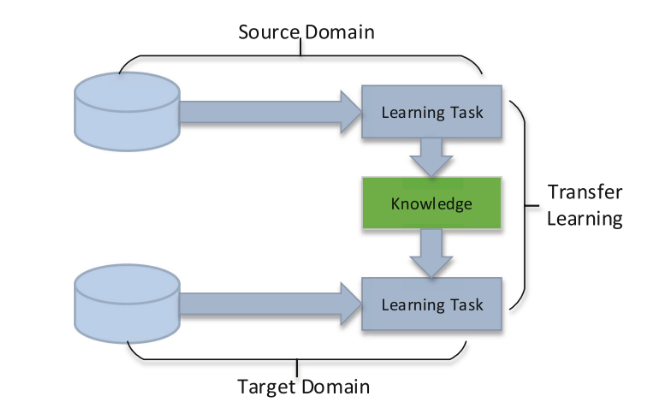
\includegraphics[scale=0.5]{Figures/process1.png}
		\rule{35em}{0.5pt}
	\caption[The Transfer Learning Process]{Learning process of transfer learning.}
	\label{fig:Transfer Learning Process}
\end{figure}


First of all, we give the definitions of a domain and a task respectively: A domain can be represented by D = {$\chi$, P(X)}, which contains two parts: the feature space $\chi$ and the edge probability distribution P(X) where X = {$x_1$, ..., $x_n$} $\in$ $\chi$. A task can be represented by T = {y, \emph{f(x)}}. It consists of two parts: label space \emph{y} and target prediction function \emph{f(x)}. \emph{f(x)} can also be regarded as a conditional probability function {P(y $\mid$ x)}. Then, the transfer learning can be formal defined as follows:

\emph{Definition 1 (Transfer Learning): Given a learning task $T_t$ based on $D_t$ and we can get the help from $D_s$ for the learning task $T_s$. Transfer learning aims to improve the performance of predictive function $f_T$ (·) for learning task $T_t$ by discover and transfer latent knowledge from $D_s$ and $T_s$, where $D_s$ = $D_t$ and/or $T_s$ = $T_t$. In addition, in the most case, the size of $D_s$ is much larger than the size of $D_t$, $N_s$, $N_t$.}\cite{tan2018survey}

Transfer learning offers the capacity to transfer information from a simulated domain to a real-world setting. Transfer learning works well when data from various feature spaces or domains is used to train a model. Machine learning applications frequently need a significant amount of real-world data. Inadequate data may be compensated for by producing simulated data in the virtual world and applying transfer learning to bridge the gap.\cite{akhauri2020enhanced} By transferring information from a similar subject, transfer learning can boost learning. For example, knowledge in mathematics and statistics can aid in understanding of machine learning ideas. Transfer learning research has focused on adapting to new domains, applications, and methodologies throughout the previous decade. "A Survey of Transfer Learning" by Karl Weiss\cite{5288526} explicitly defines transfer learning, discusses the current state of the art, and examines transfer learning applications. In particular, we investigate the application of transfer learning in autonomous driving, with an emphasis on transfer from the different world domains.

A large amount of training data is required for a model to achieve appropriate accuracy. A large amount of training data is required for a model to achieve appropriate accuracy. Transfer Learning is one solution to this problem. Transfer learning occurs when a network or model is trained on one dataset and one task and then utilized to train on another dataset and task. When a network is trained on pictures, the earliest layers tend to learn low-level characteristics such as edges, lines, and corners. Because it occurs regardless of whatever dataset is utilized, these characteristics are referred to as universal features.
We apply the fine-tuning technique, which replaces not only the classifier but also the weights in the previous layers for weight initialization. The network is then retrained with the fresh dataset and a new classifier is added on top. It is called fine-tuning because the weights are modified from the place they were in the pre-trained network to match the new dataset rather than being trained from start. It is also possible to freeze the previous layers, which means they are no longer trainable; however, because the earlier layers consist of generic characteristics, they may be left alone. Only the more specific properties of the previous dataset are changed in this scenario to better match the new job and dataset.\cite{strömgren}

Researchers utilize transfer learning for object detection due to the scarcity of labelled data and the time necessary to label the data. Lim et al. \cite{lim_1970} used transfer learning to develop a unique strategy for accommodating limited training data examples in a certain class.This is where transfer learning will contribute to universalising the learning architecture. Using autonomous cars as the base case, we can use transfer learning to generate models for other vehicular systems. During the early stages of literature review, we can assert that transfer learning can be used in the proposed system and modularized during the lane detection phase for a particular system as well as transferring model knowledge to other vehicular systems. 
% % Chapter 3

\chapter{Related Work} % Main chapter title

\label{Chapter3} % For referencing the chapter elsewhere, use \ref{Chapter1} 

\lhead{Chapter 3. \emph{Related Work}} % This is for the header on each page - perhaps a shortened title

%------------------------

---------------------------------------------------------------

This section describes the most current deep-learning-based lane detecting systems. Current approaches may be grouped into three groups depending on the strategy of line form description: traditional methods, Convolutional Neural Network (CNN) models, Deep Learning (DL) methods.


\section{Traditional Methods}

Traditional Methods in car lane detection rely on a combination of highly specialized, refined features and heuristics to along with the region of interest concepts to enable detection.\cite{neven_towards_2018} Mathematical implementations such as Canny edge Detection, Hough Transformations as well as Sobel filter methods are used to detect the lane lines. The Canny edge detector technique is utilized to identify road edges, while the Hough transformation method can be defined as a process which finds and shows shapes in the particular image input.\cite{wang_lanenet_2018} To decrease noise and improve accuracy, the region of interest (ROI) is computed in real time. It is also effective for shortening the execution time.  Sobel filter method is usually used as a edge detection algorithm in image processing where the gray scale colour space is closer to the edge information in the actual image.\cite{fong_real-time_2020}\cite{kamci_lane_2019} Recent research has been done in refined methods such as colour based methodologies\cite{1505186}, structural features\cite{neven2017fast}, the bar filter\cite{teng2010}, ridge features\cite{lopez2010} along with a Hough Transform\cite{liu2010}\cite{5548087}\cite{assidiq_real_2008} or particle or Kalman filters\cite{4459093}\cite{danescu2009}\cite{teng2010}. 
Hur et al.,(2013)\cite{hur_multi-lane_2013} proposed a new multi-lane detection algorithm which detects four lane marks, including driving lane marks and adjacent lane marks. In the study, they have included support for cross-sections as well as non-parallel lanes by implementing Conditional Random Fields (CRFs), which are strong models for solving multiple association tasks. 

\section{Convolutional Neural Network Models}
Convolutional neural networks (CNNs) are used in recent state-of-the-art lane identification techniques to train deep learning models using popular benchmarks such as TuSimple\cite{noauthor_tusimple_2021} and CULane\cite{CULane_Dataset}. While each of the following discussed models performs exceptionally well on train and test inputs from the same dataset, its performance suffers dramatically when tested on unknown datasets from various contexts.
Hang et al.,(2019)\cite{lo_multi-class_2019} proposes two CNN techniques which are Feature Size
Selection (FSS) and Degressive Dilation Block (DD Block). They introduced these methodologies to modify the existing semantic segmentation networks. EDANet\cite{lo2019efficient} was chosen as their baseline architecture due to it having a good balance between the efficiency and performance speed for a well defined autonomous driving model. For proper lane localisation, precise geographical information is required and so EDANet features three downsampling processes, whereas most CNNs contain multiple downsampling layers. The modified network achieved an Mean Intersection over Union (MIoU) score of 75.0 on the ITRI dataset.\cite{lo_multi-class_2019} 

Liu et al.,(2020)\cite{liu_lane_2020} present a method for increasing the environmental flexibility of the lane detector using Generative Adversarial Networks (GANs) to produce pictures in low-light circumstances. Their suggested approach is divided into three parts: the SIM-CycleGAN, the light conditions style transfer, and the lane identification network. They used ERFNet to evaluate their approaches on the lane detection benchmark CULane and received a 73.9 F-1 score.
Researchers have also worked on formulating feed-forward networks (FFNs) for parameter predictions which are then passed on and trained with a Hungarian fitting loss.\cite{liu_end--end_2020} This end-to-end model outputs parameters of a lane shape model based on a network which is built with a transformer encoder to capture and learn richer features from the images.  
Spatial CNN (SCNN) is a modified convolutional network proposed by Pan et al., (2018)\cite{pan_spatial_2017} that generalizes typical deep layer-by-layer convolutions to slice-by-slice convolutions inside feature maps, allowing message passings across pixels across rows and columns in a layer. They apply SCNN on Cityscapes dataset with an Intersection over Union (IoU) of 71.6 outperforming Recurrent Neural Network (RNN) based ReNet by 8.7\%. 

Chng et al.,(2020)\cite{chng_roneld_2020}, introduces a technique for identifying, tracking, and optimizing active lanes using deep learning probability map outputs using real-time robust neural network output enhancement for active lane identification (RONELD). The network adaptively extracts lane points from probability map outputs, then detects curved and straight lanes before applying weighted least squares linear regression on straight lanes to correct damaged lane edges caused by edge map fragmentation in actual pictures. Finally, they postulate genuine active lanes by tracking previous frames. On cross-dataset validation tests, experimental results show an up to two-fold boost in accuracy when using RONELD.  
According to Wang et al.(2021)\cite{wang_multitask_2021}, even if the accuracy of lane line prediction is improving, the capacity of lane markings to localize is rather limited, especially when the lane marking location is remote in nature. They offer a multi-task strategy that combines CNN's network to model semantic information with the high localization ability supplied by handmade features and forecasts the position of the vanishing line. The accuracy of location and network convergence speed are increased by incorporating segmentation, unique handcrafted characteristics, and fitting. Their network outperforms SCNN, ReNet by a huge margin on the benchmark dataset CuLane with a F-1 score of 69.6 for Curved Lanes. 

\section{Deep Learning Methods}

Xu et al.,(2020)\cite{xu_curvelane-nas_2020} provide CurveLane-NAS, a novel lane-sensitive architecture search framework for autonomously collecting both long-ranged coherent and accurate short-range curve information. It has three search modules: a feature fusion search module to investigate a better fusion of the local and global context for multi-level hierarchy features; an elastic backbone search module to investigate an efficient feature extractor with good semantics and latency; and an adaptive point blending module to investigate a multi-level post-processing refinement strategy to combine multi-scale head prediction. They also introduce the benchmark called CurveLanes\cite{soulmateb_soulmatebcurvelanes_2021} to include the most problematic curve lanes. It has 150K photos and 680K labels and their procedure model achieves an F1-score of 80.0. 
Zhang et al.,(2018)\cite{zhang_end_2018} present a deep learning model, Global Convolution Networks (GCN), that handles both classification and localization challenges in semantic lane segmentation. To attain cutting-edge performance, they employ color-based segmentation, a residual-based boundary refinement, and Adam optimization. 

Researchers\cite{liu_condlanenet_2021} introduce CondLaneNet which is a unique top-to-down lane identification framework that identifies lane instances first and then predicts the line shape for each instance dynamically. The research provides a conditional lane detection technique based on conditional convolution and row-wise formulation to re-solve the lane instance-level discriminating problem. Furthermore, they also introduce the Recurrent Instance Module (RIM) to address the issue of recognizing lane lines with complicated topologies, such as dense lines and fork lines. The advantage from their method is the real-time efficiency and end-to-end pipeline, which requires minimum post-processing. Furthermore, this approach combines accuracy and efficiency, as seen by a 78.14 F1 score and 220 FPS on CULane\cite{CULane_Dataset}. LaneNet is a deep learning module which has been presented by Neven et al.,(2018)\cite{neven_towards_2018} which performs end-to-end lane detection by combining binary lane segmentation with a clustering loss function designed for one-shot instance segmentation. the network generates parameters of a perspective transformation where lane fitting is optimal. LaneNet achieves an accuracy of 96.4\% on the TuSimple dataset.      

Yoo et al.,(2020)\cite{yoo_end--end_2020} view the problem not belonging to the instance segmentation field but as finding the set of horizontal locations of each lane marker in the input image. They propose a deep learning model which has been combined with lane marker-wise horizontal reduction modules (HRMs) on top of a end-to-end lane marker detection architecture (E2E-LMD). They achieve an F-1 socre of 74.0 against the benchmark CuLane and 96.06\% accuracy for TuSimple. Zou et al.,(2020)\cite{zou_robust_2020} examine lane detection utilizing numerous frames from a continuous driving scenario and propose a hybrid deep architecture that combines the convolutional neural network (CNN) and the recurrent neural network (RNN) (RNN). A CNN block extracts information from each frame, and the CNN features of numerous continuous frames with the property of time-series are then sent into the RNN block for feature learning and lane prediction.

Wang et al.,(2018)\cite{wang_lanenet_2018} devised a lane detecting approach that is comprised of two deep neural networks. The lane edge proposal network uses the initial input image of a vehicle's front view to generate a lane edge proposal map. The lane line localization network is then in charge of determining the position of each lane given by the lane edge map. The use of a deep neural network endows the method with great robustness, and the two-stage detection pipeline reduces computational cost and allows the lane line localization network to be trained in a manner that combines supervised and weekly supervised learning, resulting in a significant reduction in the cost of labeling training data.
% % Chapter 4

\chapter{Proposed Methodology} % Main chapter title

\label{Chapter4} % For referencing the chapter elsewhere, use \ref{Chapter1} 

\lhead{Chapter 4. \emph{Proposed Methodology}} % This is for the header on each page - perhaps a shortened title

%------------------------
---------------------------------------------------------------

\section{CondLaneNet}

Given an input image I $\in$  {$R^{C \times H \times W}$}, the goal of our 
CondLaneNet is to predict a collection of lanes L = {$l_1$ , $l_2$ , ..., $l_N$}, 
where N is the total number of lanes. Generally, each lane $l_k$ is represented by an ordered set of coordinates as follows.
\begin{equation}
l_k = [(x_{k1} , y_{k1} ), (x_{k2} , y_{k2} ), ..., (x_{kN_k} , y_{kN_k} )]
\label{eqn:Einstein}
\end{equation}
 Where k is the index of lane and $N_k$ is the max number of sample points of the $k^{th}$ lane.
 
We describe a conditional lane detection method based on conditional convolution, which is a convolution operation with adjustable kernel parameters that focuses on instance-level discrimination abilities. The conditional detection method consists of two steps: instance detection and shape prediction. The instance detection stage predicts the object instance and regresses a set of dynamic kernel parameters for each instance. In the shape prediction step, conditional convolutions are utilized to determine the instance shape. The dynamic kernel settings are used in this method. Because each instance corresponds to a set of dynamic kernel parameters, shapes may be predicted instance by instance. Our conditional lane
detection strategy improves shape prediction and instance
detection to address the above problems.
\begin{figure}[htbp]
	\centering
		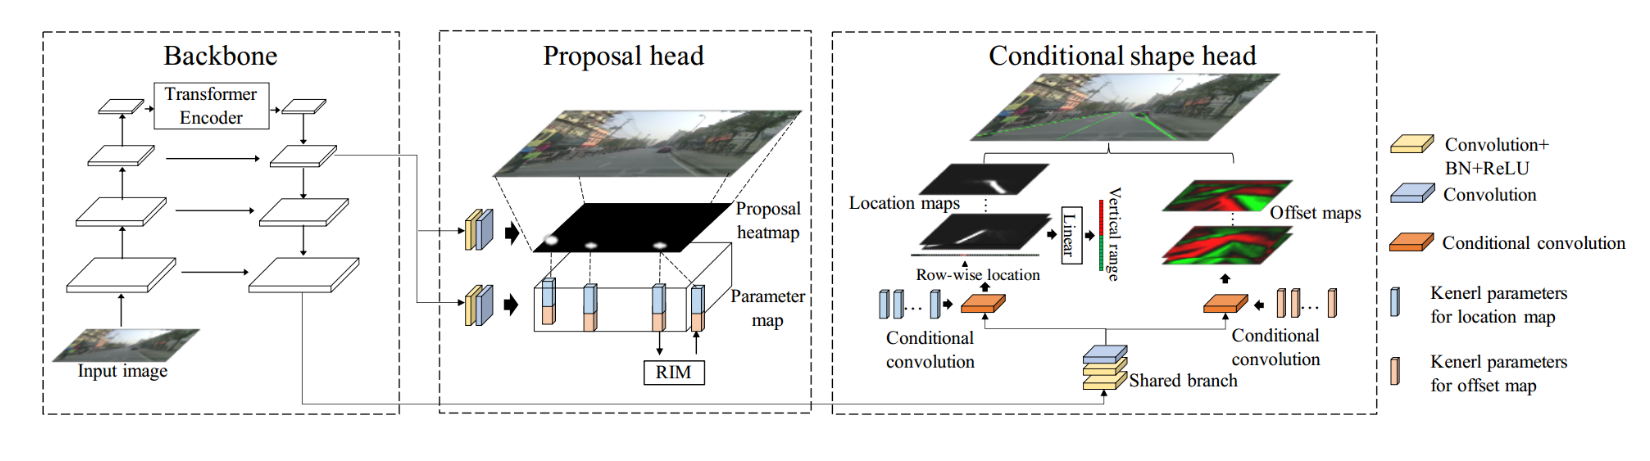
\includegraphics[scale=0.3]{Figures/condlane.png}
		\rule{35em}{0.5pt}
	\caption[CondLaneNet Architecture]{The CondLaneNet Architecture.}
	\label{fig:CondLaneNet Architecture}
\end{figure}

Figure 2 shows how we update the row-wise formulation [30] to estimate the line shape based on our conditional shape head. Based on the previous of the line shape, we estimate the lane position on each row and then aggregate the locations to produce the lane line in the order from bottom to top. Our row-wise formulation is made up of three parts: the row-wise location, the vertical range, and the offset map. Most row-wise detection algorithms rely on the first two outputs. In addition, we anticipate an offset map as the third output for additional tuning.

Each row on the location map includes an abscissa indicating the position of the lane line.
A basic way for obtaining row-wise location is to process the X-classes categorization in each row. The row-wise location is found in inference time by selecting the most responsive abscissa in each row. However, it is usual for the line to be located between the two grids, and both grids should have a strong response. To address this issue, we propose the following formulation.
We anticipate the likelihood of the lane line appearing in each grid for each row.

\begin{equation}
p_i = softmax(f^i_loc)
\label{eqn:Softmax Function}
\end{equation}

Where \emph{i} represents the \emph{ith}, is the feature vector of the \emph{ith} row of location map $f_loc$ , \emph{$p_i$} is the probability vector for the \emph{ith} row. The final row-wise location is defined as the expected abscissa.

\begin{equation}
E(x _i) = \sum_{j} j \times p_{ij}
\label{eqn:Softmax Function}
\end{equation}

Where \emph{E($x_i$)} is the expected abscissa, \emph{$p_{ij}$} is the probability of the lane line passing through the coordinate \emph{(j, i)}.

In the training phase, L1-loss is applied.

The vertical lane range is determined by
row-wisely predicting whether the lane line passes through
the current row, as is shown in Figure 4. We add a linear
layer and perform binary-classification row by row. We use
the feature vector of each row in the location map as the
input. The softmax-cross-entropy loss is adopted to guide
the training process.

\begin{equation}
E(x _i) = \sum_{j} j \times p_{ij}
\label{eqn:Softmax Function}
\end{equation}


\begin{figure}[htbp]
	\centering
		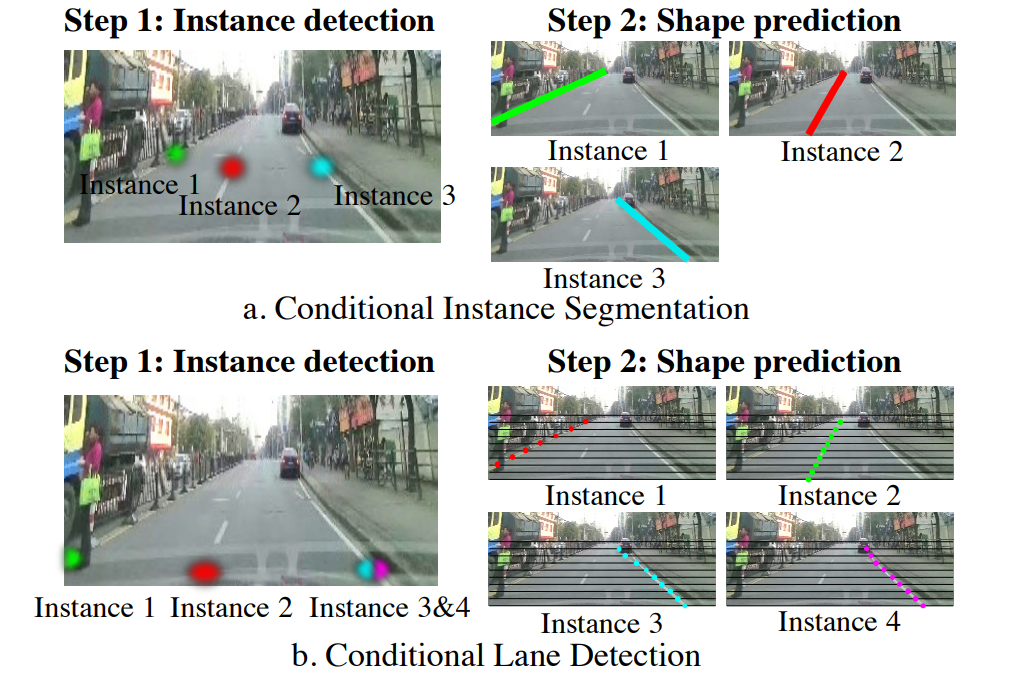
\includegraphics[scale=0.4]{Figures/condlaneprocess.png}
		\rule{35em}{0.5pt}
	\caption[The CondLaneNet Lane detection Process]{The CondLaneNet Lane detection process.}
	\label{fig:The CondLaneNet Lane Detection Process}
\end{figure}

The row-wise location defined in Equation 3
points to the abscissa of the vertex on the left side of the
grid, rather than the precise location. Thus, we add the off-
set map to predict the offset in the horizontal direction near
the row-wise location for each row.


We design the proposal head for instance detection, as is
shown in Figure 2. For general conditional instance seg-
mentation methods [35, 38], the instance is detected in anend-to-end pipeline by predicting the central of each object.
However, it is hard to predict the central for the slender and
curved lines because the visual characteristic of the line cen-
tral is not obvious.
We detect the lane instance by detecting the proposal
point located at the start point of the line. The start point has
a more clear definition and more obvious visual character-
istic than the central. We follow CenterNet [5] and predict
a proposal heatmap to detect the proposal points.


In the proposal head described above, each proposal
point is bound to a lane instance. However, in practice, mul-
tiple lane lines can fall in the same proposal point such as
the fork lanes. To deal with the above cases, we propose the
Recurrent Instance Module(RIM).

he structure of the proposed RIM is shown in Figure 5.
Based on LSTM(Long Short-term Memory) [9], the RIM
recurrently predicts a state vector s i and a kernel parame-
ter vector k i . We define s i as two-dimensional logits that
indicate two states: “continue” or “stop”. The vector k i
contains the kernel parameters for subsequent instance-wise
dynamic convolution. In the inference phase, the RIM re-
currently predicts the lane-wise kernel parameters bound to
the same proposal point until the state is “stop”.

he overall architecture is shown in Figure 2. We adopt
ResNet [8] as the backbone and add a standard FPN [23]
module to provide integrated multi-scale features. The pro-
posal head detects the lane instances by predicting the pro-
posal heatmap of shape 1 × H p × W p . Meanwhile, a pa-
rameter map of shape C p × H p × W p that contains the
dynamic kernel parameters is predicted. For the instance
with the proposal point located at (x p , y p ), the correspond-
ing dynamic kernel parameters are contained in the C p di-
mensional kernel feature vector at (x p , y p ) on the parameter
map. Further, given the kernel feature vector, the RIM re-
currently predicts the dynamic kernel parameters. Finally,
the conditional shape head predicts the line shape instance-
wisely conditioned on the dynamic kernel parameters.

Our framework requires a strong capability of context
feature fusion. For example, the prediction of the proposal
point is based on the features of the entire lane line whichgenerally has an elongated shape and long-range. There-
fore, we add a transformer encoder structure to the last layer
of the backbone for the fusion of contextual information.
We retain the two-dimensional spatial features in the en-
coder layer and use convolutions for feature extraction. The
structure of the transformer encoder used in our framework
is shown in Figure 6.

\section{ERFNet Model}

In this section, we introduce our efficient architecture for
real-time semantic segmentation. Our proposal aims at solving
an efficiency limitation that is inherently present in commonly
adopted versions of the residual layer, which is used in several
recent ConvNets that achieve top accuracy in classification [6]
and segmentation tasks [8][20][11]. By solving this limitation,
we manage to develop a semantic segmentation architecture
that makes a much more efficient use of parameters compared
to existing architectures, allowing our network to obtain a very
high segmentation accuracy while keeping top efficiency in
order to satisfy the constraints present in IV applications.

\begin{figure}[htbp]
	\centering
		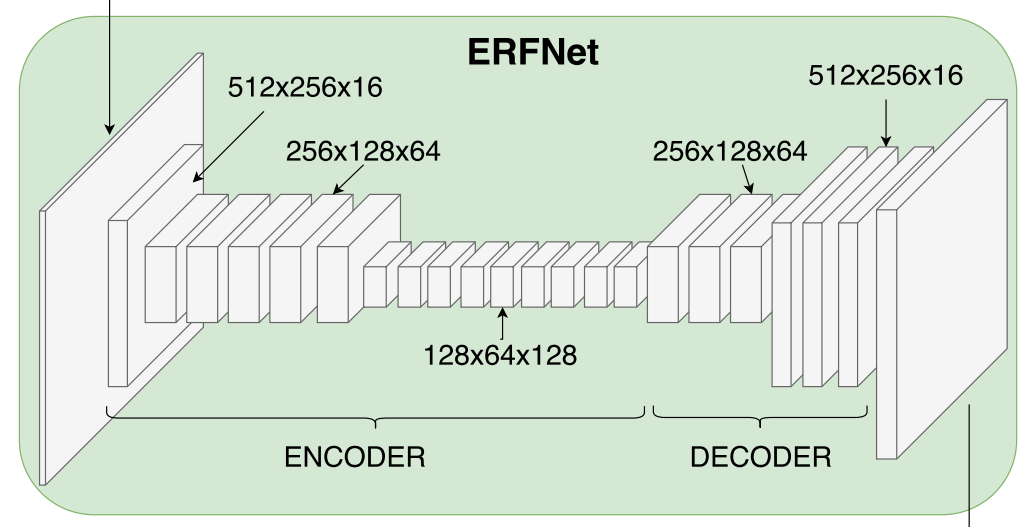
\includegraphics[scale=0.4]{Figures/erfnet.png}
		\rule{35em}{0.5pt}
	\caption[The ERFNet Model Architecture]{The ERFNet Model Architecture.}
	\label{fig:The ERFNet Model Architecture}
\end{figure}
Residual layers [6] have the property of allowing convolu-
tional layers to approximate residual functions, as the output
vector y of a layer vector input x becomes:
y = F(x, {W i }) + W s x
(1)
where W s is usually an identity mapping and F(x, {W i })
represents the residual mapping to be learned. This residual
formulation facilitates learning and significantly reduces the
degradation problem present in architectures that stack a large
amount of layers [6]. The original work proposes two instances
of this residual layer: the non-bottleneck design with two 3x3
convolutions as depicted in Fig. 2 (a), or the bottleneck version
as depicted in Fig. 2 (b). Both versions have similar number
of parameters and almost equivalent accuracy. However, the
bottleneck requires less computational resources and these
scale in a more economical way as depth increases. Hence, the
bottleneck design has been commonly adopted in state-of-the-
art networks [6][8][20][11]. However, it has been reported that
non-bottleneck ResNets gain more accuracy from increased
depth than the bottleneck versions, which indicates that they
are not entirely equivalent and that the bottleneck design still
suffers from the degradation problem [6][7][21].
We propose to redesign the non-bottleneck residual module
in a more optimal way by entirely using convolutions with 1D
filters (Fig. 2 (c)). As demonstrated in [22], any 2D filter can
be represented by a combination of 1D filters in the following
h
v
way. Let W $\in$ R C×d ×d ×F denote the weights of a typical
2D convolutional layer, where C is the number of input
planes, F is the number of output planes (feature maps) and
d h ×d v represents the kernel size of each feature map (typically
d h $\equiv$ d v $\equiv$ d). Let b $\in$ R F be the vector representing
h
v
the bias term for each filter and f i $\in$ R d ×d represent the
ith kernel in the layer. Common approaches first learn these
filters from data and then find low-rank approximations as
a post-processing step [23]. However, this approach requires
additional fine tuning and the resulting filters may not be
separable. Instead, [24] demonstrates that it is possible to relax
the rank-1 constraint and essentially rewrite f i as a linear
combination of 1D filters:

Considering an equal kernel size d for simplicity, it is trivial
to see that the decomposition reduces W 2D$\in$R C×d×d×F
of any 2D convolution into a pair of W 1D$\in$R C×d×F ,
resulting the equivalent dimensions of each 1D pair in dim =
2 × (C × d × F ). Therefore, this factorization can be ap-
plied to reduce the 3x3 convolutions on the original residual
modules. While larger filters would be more benefited by
this decomposition, applying it on 3x3 convolutions already
yields a 33\% reduction in parameters and further increases its
computational efficiency.
By leveraging this decomposition, we propose a new imple-
mentation of the residual layer that makes use of the described
1D factorization to accelerate and reduce the parameters of the
original non-bottleneck layer. We refer to this proposed mod-
ule as “non-bottleneck-1D” (non-bt-1D), which is depicted in
Fig. 2 (c). This module is faster (as in computation time)
and has less parameters than the bottleneck design, while
keeping a learning capacity and accuracy equivalent to the
non-bottleneck one. Table I summarizes the total dimensions
of the weights on the convolutions of every residual block,
comparing original ones with our proposed 1D factorizations.
Both non-bottleneck and bottleneck implementations can be
factorized into 1D kernels. However, the non-bottleneck design
is clearly more benefited, by receiving a direct 33\% reduction
in both convolutions and greatly accelerating its execution
time. As demonstrated in our experiments, this acceleration
even makes it faster than the bottleneck design, whose original
purpose according to [6] was to accelerate training time.

n this work, our main motivation is to obtain an architecture
that gets the best possible trade-off between accuracy and
efficiency. With this target in mind, we followed the current
trend of using convolutions with residual connections as the
core elements of our architecture, in order to leverage their
success in classification and segmentation problems. However,
as stated in the previous section, the commonly used residual
layers inherited some limitations in terms of learning capacity
and efficiency, which we aimed to minimize with our proposed
non-bottleneck-1D (non-bt-1D) layer. This novel block, that
leverages residual connections with factorized convolutions
and combines the strengths of bottleneck and non-bottleneck
designs, is the core of our architecture. Our network is de-
signed by stacking sequentially the proposed non-bt-1D layers
in a way that best leverages their learning performance and
efficiency.
Our architecture is fully depicted in Table II. We follow an
encoder-decoder architecture like SegNet [16] and ENet [11].
Contrary to architectures like FCN [5], where feature maps
from different layers need to be fused to obtain a fine-grain
output, our approach follows a more sequential architecture
based on an encoder segment producing downsampled feature
maps and a subsequent decoder segment that upsamples the
feature maps to match input resolution. Long-range skip
connections between the encoder and the decoder have been
used to improve accuracy in other works like [26]. However,
our architecture does not include these long-range skip connec-
tions as we did not obtain any empirical improvement. Fig. 1
contains a depiction of the feature maps generated by each of
the blocks in our architecture, from the RGB image (encoder’s
input) to the pixel class probabilities (decoder’s output).
The layers from 1 to 16 in our architecture form the encoder,
composed of residual blocks and downsampling blocks. Down-
sampling (reducing the spatial resolution) has the drawback
of reducing the pixel precision (coarser outputs), but it also
has two benefits: it lets the deeper layers gather more context
(to improve classification) and it helps to reduce computation.
Therefore, to keep a good balance we perform three downsam-
plings: at layers 1, 2 and 8. Our downsampler block, inspired
by the initial block of ENet [11], performs downsampling by
concatenating the parallel outputs of a single 3x3 convolution with stride 2 and a Max-Pooling module. ENet uses it only
as the initial block to perform early downsampling, but we
use it in all the downsampling layers that are present in
our architecture. Additionally, we also interleave some dilated
convolutions [27] in our non-bt-1D layers to gather more
context, which led to an improvement in accuracy in our
experiments. This technique has been proven more effective
(in terms of computational cost and parameters) than using
larger kernel sizes. In Table II, for those blocks that are
marked as “dilated”, we change the second pair of 3x1 and
1x3 convolutions for a pair of dilated 1D convolutions. We
also include Dropout [28] in all our non-bt-1D layers as a
regularization measure, although we triplicate its probability
(0.3 in contrast to 0.1 used in ENet), as this yielded better
results in our architecture.
The decoder segment is composed of the layers from 17
to 23. Its main task is to upsample the encoder’s feature
maps to match the input resolution. While SegNet had a
relatively symmetric encoder-decoder shape (i.e. decoder of
equal size to encoder), we follow a similar strategy to ENet
in having a small decoder whose only purpose is to upsample
the encoder’s output by fine-tuning the details. In contrast to
SegNet and ENet, we do not use max-unpooling operation
for the upsampling. Instead, our architecture includes simple
deconvolution layers with stride 2 (also known as transposed
convolutions or full-convolutions). The main advantage of
using deconvolutions is not requiring to share the pooling
indexes from the encoder. Therefore, deconvolutions simplify
memory and computation requirements. In addition, we em-
pirically obtained similar (or slightly better) accuracy.
\section{ERF-CondLaneNet}
% % Chapter 5

\chapter{Experiments and Results} % Main chapter title

\label{Chapter5} % For referencing the chapter elsewhere, use \ref{Chapter1} 

\lhead{Chapter 5. \emph{Experiments and Results}} % This is for the header on each page - perhaps a shortened title

%------------------------

------------------------------------------------------------------------------------------------

\section{Datasets}


\begin{table}[]
\centering
\resizebox{\textwidth}{!}{%
\begin{tabular}{lllll}
\hline
\textbf{Dataset} & \textbf{Train} & \textbf{Validation} & \textbf{Test} & \textbf{Road Type} \\ \hline
CurvedLanes & 100K & 20K & 30K & Curved Lane Type Urban Roads \\ \hline
CuLane & 88.9K & 9.7K & 34.7K & Straight \& Curved Lane Mix  \\ \hline
TuSimple & 3.3K & 0.4K & 2.8K & Straight Lane type Highway Roads \\ \hline
\end{tabular}%
}
\caption{}
\label{tab:my-table}
\end{table}

To extensively evaluate the proposed method, we conducte
experiments on three benchmarks: CurveLanes [39], CU-
Lane [28], and TuSimple [36]. CurveLanes is a recently
proposed benchmark with cases of complex topologies such
as fork lines and dense lines. CULane is a widely used large
lane detection dataset with 9 different scenarios. TuSimple
is another widely used dataset of highway driving scenes.
The details of the three datasets are shown in Tab. 1.

To extensively evaluate the proposed method, we conducte
experiments on three benchmarks: CurveLanes [39], CU-
Lane [28], and TuSimple [36]. CurveLanes is a recently
proposed benchmark with cases of complex topologies such
as fork lines and dense lines. CULane is a widely used large
lane detection dataset with 9 different scenarios. TuSimple
is another widely used dataset of highway driving scenes.
The details of the three datasets are shown in Tab. 1.




\section{Initial Training}
If you are familiar with \LaTeX{}, then you can familiarise yourself with the contents of the Zip file and the directory structure and then place your own information into the `\texttt{Thesis.cls}' file. Section \ref{FillingFile} on page \pageref{FillingFile} tells you how to do this. Make sure you read section \ref{ThesisConventions} about thesis conventions to get the most out of this template and then get started with the `\texttt{Thesis.tex}' file straightaway.

If you are new to \LaTeX{} it is recommended that you carry on reading through the rest of the information in this document.

\LaTeX{} is not a WYSIWYG (What You See is What You Get) program, unlike word processors such as Microsoft Word or Apple's Pages. Instead, a document written for \LaTeX{} is actually a simple, plain text file that contains \emph{no formatting}. You tell \LaTeX{} how you want the formatting in the finished document by writing in simple commands amongst the text, for example, if I want to use \textit{italic text for emphasis}, I write the `$\backslash$\texttt{textit}\{\}' command and put the text I want in italics in between the curly braces. This means that \LaTeX{} is a ``mark-up'' language, very much like HTML.

\subsection{A (not so short) Introduction to \LaTeX{}}

If you are new to \LaTeX{}, there is a very good eBook -- freely available online as a PDF file -- called, ``The Not So Short Introduction to \LaTeX{}''. The book's title is typically shortened to just ``lshort''. You can download the latest version (as it is occasionally updated) from here:\\
\href{http://www.ctan.org/tex-archive/info/lshort/english/lshort.pdf}{\texttt{http://www.ctan.org/tex-archive/info/lshort/english/lshort.pdf}}

It is also available in several other languages. Find yours from the list on this page:\\
\href{http://www.ctan.org/tex-archive/info/lshort/}{\texttt{http://www.ctan.org/tex-archive/info/lshort/}}

It is recommended to take a little time out to learn how to use \LaTeX{} by creating several, small `test' documents. Making the effort now means you're not stuck learning the system when what you \emph{really} need to be doing is writing your thesis.

\subsection{A Short Math Guide for \LaTeX{}}

If you are writing a technical or mathematical thesis, then you may want to read the document by the AMS (American Mathematical Society) called, ``A Short Math Guide for \LaTeX{}''. It can be found online here:\\
\href{http://www.ams.org/tex/amslatex.html}{\texttt{http://www.ams.org/tex/amslatex.html}}\\
under the ``Additional Documentation'' section towards the bottom of the page.

\subsection{Common \LaTeX{} Math Symbols}
There are a multitude of mathematical symbols available for \LaTeX{} and it would take a great effort to learn the commands for them all. The most common ones you are likely to use are shown on this page:\\
\href{http://www.sunilpatel.co.uk/latexsymbols.html}{\texttt{http://www.sunilpatel.co.uk/latexsymbols.html}}

You can use this page as a reference or crib sheet, the symbols are rendered as large, high quality images so you can quickly find the \LaTeX{} command for the symbol you need.

\subsection{\LaTeX{} on a Mac}
 
The \LaTeX{} package is available for many systems including Windows, Linux and Mac OS X. The package for OS X is called MacTeX and it contains all the applications you need -- bundled together and pre-customised -- for a fully working \LaTeX{} environment and workflow.
 
MacTeX includes a dedicated \LaTeX{} IDE (Integrated Development Environment) called ``TeXShop'' for writing your `\texttt{.tex}' files and ``BibDesk'': a program to manage your references and create your bibliography section just as easily as managing songs and creating playlists in iTunes.




\section{Cross Dataset Analysis}


% % Chapter 6

\chapter{Conclusion} % Main chapter title

\label{Chapter6} % For referencing the chapter elsewhere, use \ref{Chapter1} 

\lhead{Chapter 6. \emph{Conclusion}} % This is for the header on each page - perhaps a shortened title

%------------------------

---------------------------------------------------------------
In this work, We proposed CondLaneNet, a novel top-
to-down lane detection framework that detects the lane in-
stances first and then instance-wisely predict the shapes.
Aiming to resolve the instance-level discrimination prob-
lem, we proposed the conditional lane detection strategy
based on conditional convolution and row-wise formula-
tion. Moreover, we designed RIM to cope with complex
lane line topologies such as dense lines and fork lines. Our
CondLaneNet framework refreshed the state-of-the-art per-
formance on CULane, CurveLanes, and TuSimple. More-
over, on CULane and CurveLanes, the small version of our
CondLaneNet not only surpassed other methods in accu-
racy, but also presented real-time efficiency.
\section{Future Work}
% \input{Chapters/Chapter7}

%-------------------------------------------------------------------------------
%	THESIS CONTENT - APPENDICES
%-------------------------------------------------------------------------------

\addtocontents{toc}{\vspace{2em}} % Add a gap in the Contents, for aesthetics

\appendix % Cue to tell LaTeX that the following 'chapters' are Appendices

% Include the appendices of the thesis as separate files from the Appendices
% folder
% Uncomment the lines as you write the Appendices

% Appendix A

\chapter{Appendix Title Here} % Main appendix title

\label{AppendixA} % For referencing this appendix elsewhere, use \ref{AppendixA}

\lhead{Appendix A. \emph{Appendix Title Here}} % This is for the header on each page - perhaps a shortened title

Write your Appendix content here.
%\input{Appendices/AppendixB}
%\input{Appendices/AppendixC}

\addtocontents{toc}{\vspace{2em}} % Add a gap in the Contents, for aesthetics

\backmatter

%-------------------------------------------------------------------------------
%	BIBLIOGRAPHY
%-------------------------------------------------------------------------------

\label{Bibliography}

\lhead{\emph{Bibliography}} % Change the page header to say "Bibliography"

\printbibliography

\end{document}
